\documentclass{article}
\usepackage{tikz}

\begin{document}
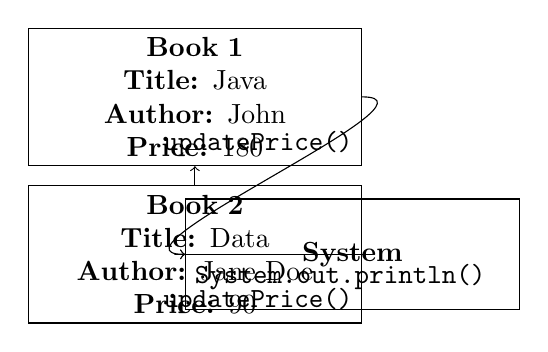
\begin{tikzpicture}[node distance=2cm, auto]
    % Define the styles for each node
    \tikzstyle{book} = [rectangle, draw, text width=4cm, text centered, minimum height=4em]
    \tikzstyle{system} = [rectangle, draw, text width=4cm, text centered, minimum height=4em]
    
    % Create the nodes for each book
    \node [book] (book1) {
        \textbf{Book 1}\\
        \textbf{Title:} Java\\
        \textbf{Author:} John\\
        \textbf{Price:} 180
    };
    \node [book, below of=book1] (book2) {
        \textbf{Book 2}\\
        \textbf{Title:} Data\\
        \textbf{Author:} Jane Doe\\
        \textbf{Price:} 90
    };
    
    % Create the node for the system
    \node [system, right of=book2] (system) {\textbf{System}};
    
    % Draw the arrows between the nodes
    \draw [->] (book1) to [out=0, in=180] (system);
    \draw [->] (book2) to [out=0, in=180] (system);
    \draw [<-] (book1) to [out=270, in=90] (book2);
    
    % Add the labels for the arrows
    \node [below right] at (system.west) {\texttt{System.out.println()}};
    \node [above left] at (book1.south east) {\texttt{updatePrice()}};
    \node [above left] at (book2.south east) {\texttt{updatePrice()}};
\end{tikzpicture}
\end{document}
